\subsection{Algoritmo implementado}

Sea G=(V,E) un grafo simple, la heuristica de busqueda local propuesta genera una solucion inicial valida, es decir un V' $\subseteq$ V que es dominante e independiente (CID), de dos formas:
\begin{enumerate}
	\item \textbf{Heuristica constructiva golosa}: procedimiento descripto en el ejercicio anterior.
    \item \textbf{Procedimiento BFS modificado}: detallado a continuación.

\end{enumerate}

\subsubsection{Procedimiento BFS modificado}
Partimos de incluir un vertice inicial $v$ a $V'$ y luego vamos a ir agregando vertices a $V'$ determinando si el vertice analizado debe incluirse en $V'$.
El BFS modificado funciona de la siguiente manera:

\begin{codesnippet}
Los vertices estan numerados de 0 a n-1.

Creamos un vector, llamado solucionInicial, de tamaño n para guardar el estado de los 
vertices (si fue VISITADO o no)

Creamos un vector de tamaño n en donde para cada posicion guardamos si 
pertence al CID (INCLUIDO o no)

Al vertice inicial v lo ponemos como VISITADO y INCLUIDO y lo incluimos en la cola.

Luego mientras no este vacia la cola:
    Sacamos el primer elemento de la cola (w) y lo ponemos INCLUIDO.
    Revisamos cada adyacente a w:
        Si algun adyacente esta INCLUIDO entonces hacemos w = NO INCLUIDO.
        Si el adyacente no fue VISITADO entonces lo ponemos como VISITADO y 
        lo agregamos a la cola.

Repetimos el procedimiento para el resto de las componentes conexas, empezando por 
el vertice de menor numeracion de la componente analizada.


\end{codesnippet}

A continuacion mostramos un ejemplo del recorrido BFS, en donde el vertice 0 ya fue visitado y se esta analizando sus adyacentes, en particular el vertice 1, el cual es provisoriamiente INCLUIDO:


\tikz[every node/.style={draw,circle}] {
\node[fill=blue!40, text=white] (1) at (0, 0)  { 0 };
\node[fill=red!40, text=white] (2) at (2, 0)  { 1 };
\node (5) at (4, 0)  { 3 };
\node (6) at (6, 0)  { 4 };
\node (7) at (3,-1)  { 2 };
\draw (1) edge node[above,draw=none] {} (2);
\draw (5) edge node[above,draw=none] {} (6);
\draw (2) edge node[above,draw=none] {} (7);
}

Para luego ser desmarcado debido a la presencia de un adyacente INCLUIDO, siendo la solucion generada la siguiente:

\tikz[every node/.style={draw,circle}] {
\node[fill=blue!40, text=white] (1) at (0, 0)  { 0 };
\node (2) at (2, 0)  { 1 };
\node[fill=blue!40, text=white] (5) at (4, 0)  { 3 };
\node (6) at (6, 0)  { 4 };
\node[fill=blue!40, text=white] (7) at (3,-1)  { 2 };
\draw (1) edge node[above,draw=none] {} (2);
\draw (5) edge node[above,draw=none] {} (6);
\draw (2) edge node[above,draw=none] {} (7);
}



\subsubsection{Primer Criterio de Vecindad}
El primer criterio de vecindad implementado consiste en generar soluciones vecinas a partir de quitar k vertices que pertenecen al subconjunto CID de la solucion inicial y agregar 1 vertice al subconjunto, donde k $\in \mathbb{N}$ y k $\geq$ 2. Logrando de esta manera una reduccion en el cardinal del subcojunto CID de, al menos, un vertice.

Para llevar adelante exitosamente este intercambio, debemos buscar aquellos vertices no incluidos en CID en la solucion inicial, que tengan, al menos, dos vertices adyacentes incluidos en CID, para poder incluir ese vertice en la solucion vecina y quitar sus adyacentes.

\begin{itemize}
	\item Ejemplo de un cambio 4 por 1:
    
    \tikz[every node/.style={draw,circle}] {
\node[fill=blue!40, text=white] (1) at (0, 0)  { 0 };
\node (2) at (1, -1)  { 1 };
\node[fill=blue!40, text=white] (5) at (2, -2)  { 3 };
\node[fill=blue!40, text=white] (7) at (2, 0)  { 2 };
\node[fill=blue!40, text=white] (8) at (0, -2)  { 4 };
\node (9) at (5, 0)  { 0 };
\node[fill=blue!40, text=white] (10) at (6, -1)  { 1 };
\node (11) at (7, -2)  { 3 };
\node (12) at (7, 0)  { 2 };
\node (13) at (5, -2)  { 4 };

\draw (1) edge node[above,draw=none] {} (2);
\draw (5) edge node[above,draw=none] {} (2);
\draw (2) edge node[above,draw=none] {} (7);
\draw (2) edge node[above,draw=none] {} (8);

\draw (9) edge node[above,draw=none] {} (10);
\draw (11) edge node[above,draw=none] {} (10);
\draw (10) edge node[above,draw=none] {} (12);
\draw (10) edge node[above,draw=none] {} (13);

}

\end{itemize}

Sin embargo, para lograr una solucion valida, los vertices quitados no pueden tener otros vertices adyacentes no incluidos en el subconjunto que, a su vez, no sean adyacentes al vertice agregado.

\begin{itemize}
	\item Ejemplo de solucion invalida:
    
    \tikz[every node/.style={draw,circle}] {
\node[fill=blue!40, text=white] (1) at (0, 0)  { 0 };
\node (2) at (1, -1)  { 1 };
\node[fill=blue!40, text=white] (5) at (2, -2)  { 3 };
\node[fill=blue!40, text=white] (7) at (2, 0)  { 2 };
\node[fill=blue!40, text=white] (8) at (0, -2)  { 4 };
\node (14) at (3.5, 0)  { 5 };
\node (9) at (5, 0)  { 0 };
\node[fill=blue!40, text=white] (10) at (6, -1)  { 1 };
\node (11) at (7, -2)  { 3 };
\node (12) at (7, 0)  { 2 };
\node (13) at (5, -2)  { 4 };
\node (15) at (8.5, 0)  { 5 };

\draw (1) edge node[above,draw=none] {} (2);
\draw (5) edge node[above,draw=none] {} (2);
\draw (2) edge node[above,draw=none] {} (7);
\draw (2) edge node[above,draw=none] {} (8);
\draw (7) edge node[above,draw=none] {} (14);

\draw (9) edge node[above,draw=none] {} (10);
\draw (11) edge node[above,draw=none] {} (10);
\draw (10) edge node[above,draw=none] {} (12);
\draw (10) edge node[above,draw=none] {} (13);
\draw (12) edge node[above,draw=none] {} (15);

}

\end{itemize}

El procedimiento de busqueda de los posibles soluciones vecinas funciona de la siguiente manera:

\begin{codesnippet}
Para todo vertice, u, en el Grafo:
  Creamos un vector de tamaño n, llamado solucionAuxiliar, al cual le copiamos 
  el contenido de la solucionInicial.
  Si solucionInicial[u] = NO INCLUIDO y |adyacentes a u| > 1 entonces:
     solucionAuxiliar[u] = INCLUIDO
     cantAdyacentesIncluidos = 0
     Para todo adyacente, v, de u:
         Si solucionInicial[v] = INCLUIDO entonces:
             cantAdyacentesIncluidos ++
             solucionAuxiliar[v] = NO INCLUIDO
  
  Si cantAdyacentesIncluidos > 1 entonces:
     Si esSolucion?(solucionAuxiliar) entonces:
       Buscar Nuevos Vecinos a partir de la solucionAuxiliar
       Interrumpir el ciclo
     
\end{codesnippet}

En el procedimiento descripto anteriormente falta detallar el comportamiento de la funciona auxiliar \textit{esSolucion?}, la cual sera descripta en el apartado siguiente, ya que es utilizado por ambos criterios.

\subsubsection{Segundo Criterio de Vecindad}
El segundo criterio de vecindad implementado consiste en generar soluciones vecinas a partir de quitar k vertices que pertenecen al subconjunto CID de la solucion inicial y agregar, hasta, k-1 vertices al subconjunto, donde k $\in \mathbb{N}$ y k $\geq$ 2. Logrando de esta manera, una reduccion en el cardinal del subcojunto CID de, al menos, un vertice.
El caso donde k = 2 no difere del criterio aplicado en la primer vecindad, ya que k - 1 = 1. Sin embargo a partir de k $\geq$ 3 se observa un comportamiento distinto, ya que podemos agregar k-1 vertices para "salvar" la solucion.

En este caso, para los casos no contemplados en el criterio anterior, debemos buscar vertices no incluidos en CID en la solucion inicial, que tengan, al menos k vertices adyacentes incluidos en CID, donde k$\geq$ 3, y que a su vez tengan hasta k-1 vertices que son adyacentes a los adyacentes del vertice buscado que no estan incluidos.

\begin{itemize}
	\item Ejemplo de un caso 4-2, el cual fallaba en el criterio anterior:
    
    \tikz[every node/.style={draw,circle}] {
\node[fill=blue!40, text=white] (1) at (0, 0)  { 0 };
\node (2) at (1, -1)  { 1 };
\node[fill=blue!40, text=white] (5) at (2, -2)  { 3 };
\node[fill=blue!40, text=white] (7) at (2, 0)  { 2 };
\node[fill=blue!40, text=white] (8) at (0, -2)  { 4 };
\node (14) at (3.5, 0)  { 5 };
\node (9) at (5, 0)  { 0 };
\node[fill=blue!40, text=white] (10) at (6, -1)  { 1 };
\node (11) at (7, -2)  { 3 };
\node (12) at (7, 0)  { 2 };
\node (13) at (5, -2)  { 4 };
\node[fill=blue!40, text=white] (15) at (8.5, 0)  { 5 };

\draw (1) edge node[above,draw=none] {} (2);
\draw (5) edge node[above,draw=none] {} (2);
\draw (2) edge node[above,draw=none] {} (7);
\draw (2) edge node[above,draw=none] {} (8);
\draw (7) edge node[above,draw=none] {} (14);

\draw (9) edge node[above,draw=none] {} (10);
\draw (11) edge node[above,draw=none] {} (10);
\draw (10) edge node[above,draw=none] {} (12);
\draw (10) edge node[above,draw=none] {} (13);
\draw (12) edge node[above,draw=none] {} (15);

}

\end{itemize}

\begin{itemize}
	\item Caso donde falla el segundo criterio:
    
    \tikz[every node/.style={draw,circle}] {
\node (1)[fill=blue!40, text=white] at (0, 0)  { 0 };
\node (2) at (1, -1)  { 1 };
\node (3)[fill=blue!40, text=white] at (2, 0)  { 2 };
\node (4)[fill=blue!40, text=white] at (2, -2)  { 3 };
\node (5) at (3.5, 0)  { 4 };
\node (6) at (3.5, -2)  { 5 };

\node (7) at (5, 0)  { 0 };
\node (8)[fill=blue!40, text=white] at (6, -1)  { 1 };
\node (9) at (7, 0)  { 2 };
\node (10) at (7, -2)  { 3 };
\node (11)[fill=blue!40, text=white] at (8.5, 0)  { 4 };
\node (12) at (8.5, -2)  { 5 };


\draw (1) edge node[above,draw=none] {} (2);
\draw (2) edge node[above,draw=none] {} (3);
\draw (2) edge node[above,draw=none] {} (4);
\draw (3) edge node[above,draw=none] {} (5);
\draw (4) edge node[above,draw=none] {} (6);

\draw (7) edge node[above,draw=none] {} (8);
\draw (8) edge node[above,draw=none] {} (9);
\draw (8) edge node[above,draw=none] {} (10);
\draw (9) edge node[above,draw=none] {} (11);
\draw (10) edge node[above,draw=none] {} (12);


}

\end{itemize}

El procedimiento de busqueda de los posibles soluciones vecinas funciona de la siguiente manera:

\begin{codesnippet}
Para todo vertice, u, en el Grafo:
  Creamos un vector de tamaño n, llamado solucionAuxiliar, al cual le copiamos 
  el contenido de la solucionInicial.
  Si solucionInicial[u] = NO INCLUIDO y |adyacentes a u| > 1 entonces:
     solucionAuxiliar[u] = INCLUIDO
     cantAdyacentesIncluidos = 0
     Para todo adyacente, v, de u:
         Si solucionInicial[v] = INCLUIDO entonces:
             cantAdyacentesIncluidos ++
             solucionAuxiliar[v] = NO INCLUIDO
  
  Si cantAdyacentesIncluidos > 1 entonces:
     cantCambiosPosibles = cantAdyacentesIncluidos - 2
     arreglarSolucion(solucionAuxiliar, cantCambiosPosibles)
     Si esSolucion?(solucionAuxiliar) entonces:
       Buscar Nuevos Vecinos a partir de la solucionAuxiliar
       Interrumpir el ciclo
     
\end{codesnippet}

Falta detallar los procedimientos \textit{arreglarSolucion} y \textit{esSolucion?}, los cuales se pueden realizar en una sola funcion que llameremos \textit{esSolucion?} cuyo comportamiento es el siguiente:
\begin{itemize}
	\item La funcion recibe como parametros un vector con la solucion a analizar y un entero con la cantidad de cambios posibles a realizar
	\item Miramos cada vertice del grafo, los cuales o estan INCLUIDOS o NO INCLUIDOS en el subconjunto CID.
    \item Si el vertice esta INCLUIDO, sus adyacentes NO pueden estar INCLUIDOS. En caso de encontrar algun adyacente INCLUIDO, sabemos que el subconjunto analizado no es solucion valida.
    \item Si el vertice NO esta INCLUIDO, entonces, al menos, 1 vertice adyacente tiene que estar INCLUIDO. En caso de no encontrar algun vertice adyacente INCLUIDO, tenemos dos casos:
    \begin{enumerate}
    	\item La variable entera que representa la cantidad de cambios posibles es 0. En este caso sabemos que el subconjunto analizado no es solucion valida.
        \item La variable entera que representa la cantidad de cambios posibles es mayor a 0. En este caso el vertice pasa a estar INCLUIDO en el subconjunto, manteniendose la validez de la solucion, ya que el vertice NO tiene adyacentes INCLUIDOS. Tambien reducimos la cantidad de cambios posibles en una unidad.
    \end{enumerate} 
    
    \item En pseudocodigo:
    
\end{itemize}

\begin{codesnippet}
Como entrada tenemos el vector solucionAuxiliar con la solucion a analizar y el entero 
cantCambiosPosibles, que tiene la cantidad de vertices que podemos incluir.

Creamos una variable booleana, esSolucion inicializadas en true.

Luego, para todo vertice, u, en el Grafo:
  Si solucionAuxiliar[u] = INCLUIDO y |adyacentes a u| > 0 entonces:
     Para todo adyacente, v, de u:
         Si solucionInicial[v] = INCLUIDO entonces:
             esSolucion = false
             Interrumpir el ciclo
             
  Sino Si |adyacentes a u| > 0, entonces:
       adyacenteIncluido = false
       Para todo adyacente, v, a u:
          Si solucionInicial[v] = INCLUIDO entonces:
             adyacenteIncluido = true
       Si not(adyacenteIncluido) y cantCambiosPosibles = 0 entonces:
         esSolucion = false
         Interrumpir el ciclo
       Sino Si not(adyacenteIncluido) entonces:
         solucionAuxiliar[u] = INCLUIDO
         cantCambiosPosibles --
  
  Sino entonces:
       esSolucion = (solucionAuxiliar[u] = INCLUIDO)
              
\end{codesnippet}

Es necesario aclarar que para el primer criterio de vecindad, la cantidad de cambios posibles es 0.

\subsection{Complejidad propuesta}
La estructura de datos que utilizamos para representar los grafos son vectores con listas, donde cada posicion del vector representa un vertice y las listas contienen los adyacentes a ese vertice.

A partir de los procedimientos expuestos en el punto anterior, pasamos a analizar la complejidad de la heuristica propuesta, para solo una iteracion:

\begin{enumerate}
  \item \textbf{Solucion Inicial}
    \begin{itemize}
    	\item \underline{Heuristica Golosa}: $\Theta{(n*log(n) + m)}$. Justificada anteriormente.
        \item \underline{BFS modificado}: Las cambios implementos en el BFS no alteran su complejidad original, siendo la misma $\mathcal{O}(n + m)$. \footnote{Referencia \url{https://en.wikipedia.org/wiki/Breadth-first_search}}
    \end{itemize}
  \item \textbf{Primer Criterio de Vecindad}
  
  Tenemos un ciclo que se repite $n$ veces, el cual tiene varias operaciones que se realizan internamente:
  \begin{itemize}
    \item Creacion de un vector tamaño $n$ y copia de contenido: $\Theta{(n)}$
    \item Comparaciones y Asignaciones: $\mathcal{O}(1)$
    \item Ciclo de los adyacentes, cuya complejidad, sumada a la del ciclo principal, es $\mathcal{O}(n + m)$.
    \item Complejidad de la funcion esSolucion?: $\mathcal{O}(n + m)$. Detallada en el punto 4.
  \end{itemize}
  Por lo tanto la complejidad total de este procedimiento es: $\mathcal{O}(n*(n + n + m) + n + m)$, lo cual es: $\mathcal{O}(n*(n + m))$
  
  \item \textbf{Segundo Criterio de Vecindad}
  
    Misma situacion que el punto anterior, tenemos un ciclo que se repite $n$ veces, el cual tiene varias operaciones que se realizan internamente:
  \begin{itemize}
    \item Creacion de un vector tamaño $n$ y copia de contenido: $\Theta{(n)}$
    \item Comparaciones y Asignaciones: $\mathcal{O}(1)$
    \item Ciclo de los adyacentes, cuya complejidad, sumada a la del ciclo principal, es $\mathcal{O}(n + m)$.
    \item Complejidad de la funcion esSolucion?: $\mathcal{O}(n + m)$. Detallada en el punto 4.
  \end{itemize}
  Por lo tanto la complejidad total de este procedimiento es: $\mathcal{O}(n*(n + n + m) + n + m)$, lo cual es: $\mathcal{O}(n*(n + m))$
  
  \item \textbf{Procedimiento esSolucion?}
  
    Tenemos un ciclo que se repite $n$ veces, el cual tiene varias operaciones que se realizan internamente:
  \begin{itemize}
    \item Comparaciones y Asignaciones: $\mathcal{O}(1)$
    \item Ciclo de los adyacentes, cuya complejidad, sumada a la del ciclo principal, es $\mathcal{O}(n + m)$.
  \end{itemize}
  Por lo tanto la complejidad total de este procedimiento es: $\mathcal{O}(n + m)$.
  
\end{enumerate}

Podemos concluir que la complejidad temporal de la heuristica es independiente del procedimiento utilizado para armar la solucion inicial, y que utilizando el primer o segundo criterio de vecindad la complejidad es la misma: $\mathcal{O}(n*(n + m))$.\\ 

\textbf{Cota superior para la cantidad de iteraciones:}
Sabemos que cada iteracion de las vecindades reduce, como minimo, en 1 el cardinal del subconjunto CID. Por lo tanto, si partimos de una solucion inicial en donde el cardinal del subconjunto es asistonticamente igual a la cantidad de vertices del Grafo, es posible que iteraremos hasta n-1 veces, hasta alcanzar una solucion de 1 vertice. Es evidente que este es un caso extremo, de dificil realizacion, sin embargo brinda una cota supeior a la cantidad de iteraciones.

\subsection{Experimentación computacional}

La función que utilizamos para llevar a cabo las mediciones fue \texttt{std::clock}\footnote{Referencia \url{http://en.cppreference.com/w/cpp/chrono/c/clock}}. La unidad temporal que utilizamos para este ejercicio fue nanosegundos.
La complejidad teórica calculada es de $\mathcal{O}(n*(n + m))$ para cualquier combinacion de solucion inicial y criterio de vecindad.

Para generar las instancias aleatorias utilizamos la función \texttt{std::rand}\footnote{Referencia \url{http://en.cppreference.com/w/cpp/numeric/random/rand}} con determinados intervalos de valores para la variables, para obtener instancias coherentes. El detalle de intervalos es el siguiente:

\begin{enumerate}
	\item Cantidad de nodos $n$: 2 $\leq$ $n$ $\leq$ 50.
    \item Cantidad de aristas $m$: 0 $\leq$ $m$ $\leq$ $\frac{n*(n-1)}{2}$.
    \item Se generan $m$ ejes, asegurandose la validez de los mismos, es decir que no haya ejes repetidos ni loops.
\end{enumerate}

Se generaron 500 instancias construidas de esta forma, en donde se midio no solo el tiempo de ejecucion, sino tambien el tamaño del subconjunto generado, para los 4 tipos contemplados en la heuristica:

\begin{itemize}
	\item Tipo B1: Utilizamos el BFS modificado para la solucion original, y el primer criterio de vecindad.
    \item Tipo G1: Utilizamos la heuristica golosa para la solucion original, y el primer criterio de vecindad.
    \item Tipo B2: Utilizamos el BFS modificado para la solucion original, y el segundo criterio de vecindad.
    \item Tipo G2: Utilizamos la heuristica golosa para la solucion original, y el segundo criterio de vecindad.
\end{itemize}

La medicion de tiempos de los distintos tipos, arroja los siguientes graficos para cada tipo:

\begin{enumerate}
\item \textbf{Tipo B1:}

\begin{figure}[H]
        \centering
        \begin{subfigure}[b]{0.5\textwidth}
                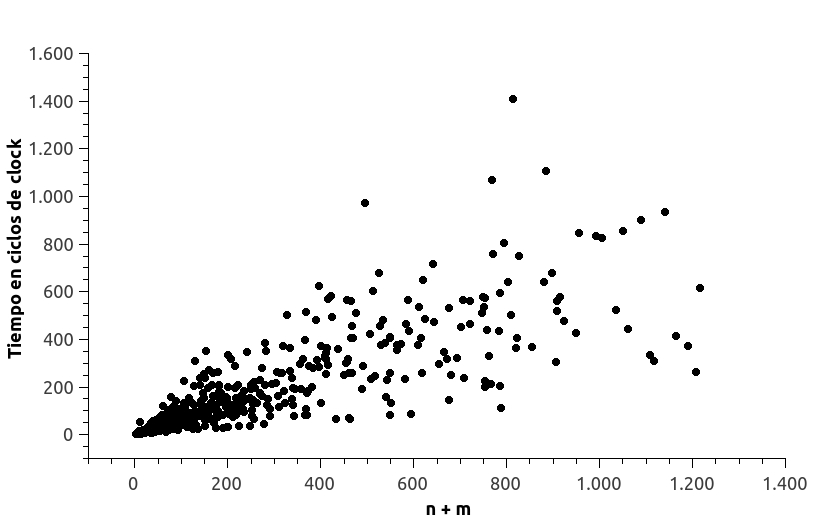
\includegraphics[width=\textwidth]{imagenes/ejer4-grafB1-1.jpg}
                \caption{Tiempos sin procesar}
        \end{subfigure}%
        ~ %add desired spacing between images, e. g. ~, \quad, \qquad, \hfill etc.
          %(or a blank line to force the subfigure onto a new line)
        \begin{subfigure}[b]{0.5\textwidth}
                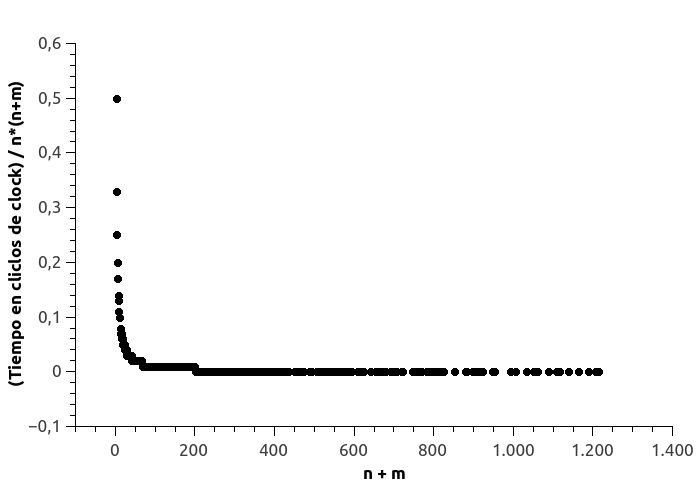
\includegraphics[width=\textwidth]{imagenes/ejer4-grafB1-2.jpg}
                \caption{figura (a) / n*(n+m)}
        \end{subfigure}
        
\end{figure}

\item \textbf{Tipo G1:}

\begin{figure}[H]
        \centering
        \begin{subfigure}[b]{0.5\textwidth}
                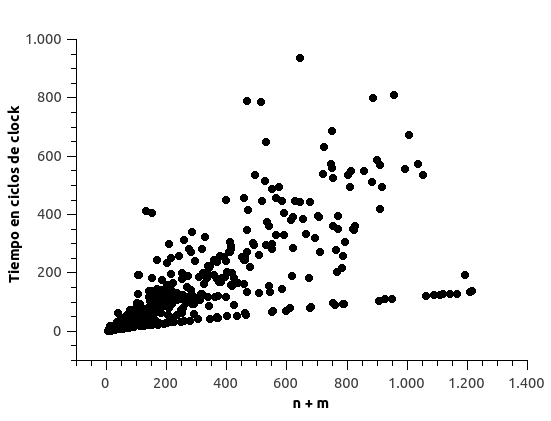
\includegraphics[width=\textwidth]{imagenes/ejer4-grafG1-1.jpg}
                \caption{Tiempos sin procesar}
        \end{subfigure}%
        ~ %add desired spacing between images, e. g. ~, \quad, \qquad, \hfill etc.
          %(or a blank line to force the subfigure onto a new line)
        \begin{subfigure}[b]{0.5\textwidth}
                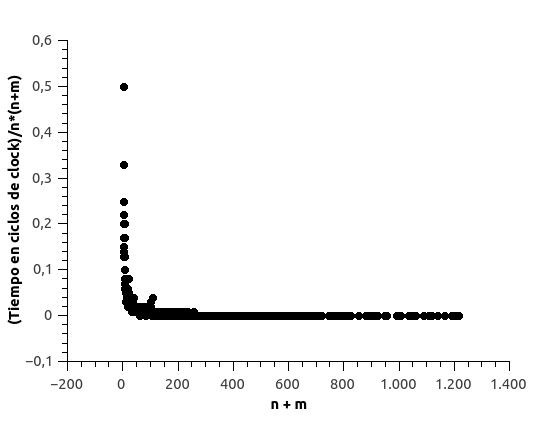
\includegraphics[width=\textwidth]{imagenes/ejer4-grafG1-2.jpg}
                \caption{figura (a) / n*(n+m)}
        \end{subfigure}
        
\end{figure}


\item \textbf{Tipo B2:}

\begin{figure}[H]
        \centering
        \begin{subfigure}[b]{0.5\textwidth}
                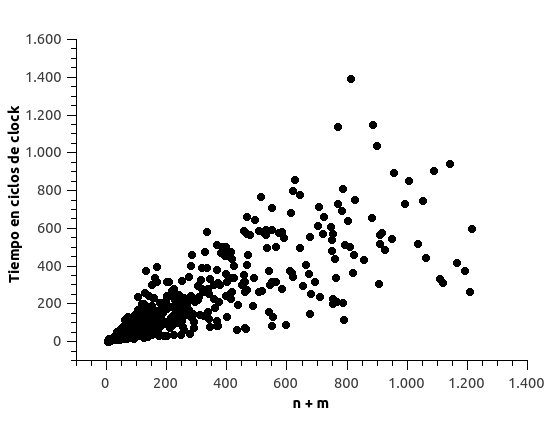
\includegraphics[width=\textwidth]{imagenes/ejer4-grafB2-1.jpg}
                \caption{Tiempos sin procesar}
        \end{subfigure}%
        ~ %add desired spacing between images, e. g. ~, \quad, \qquad, \hfill etc.
          %(or a blank line to force the subfigure onto a new line)
        \begin{subfigure}[b]{0.5\textwidth}
                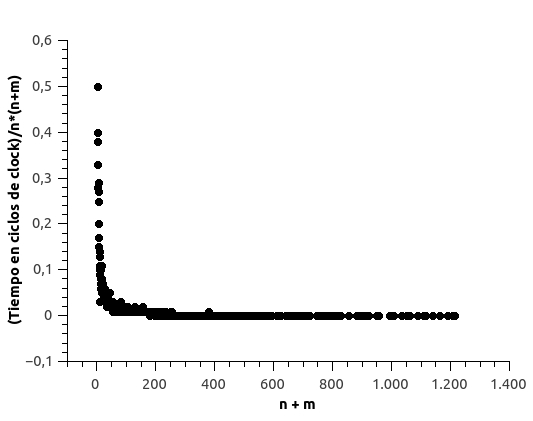
\includegraphics[width=\textwidth]{imagenes/ejer4-grafB2-2.jpg}
                \caption{figura (a) / n*(n+m)}
        \end{subfigure}
        
\end{figure}



\item \textbf{Tipo G2:}

\begin{figure}[H]
        \centering
        \begin{subfigure}[b]{0.5\textwidth}
                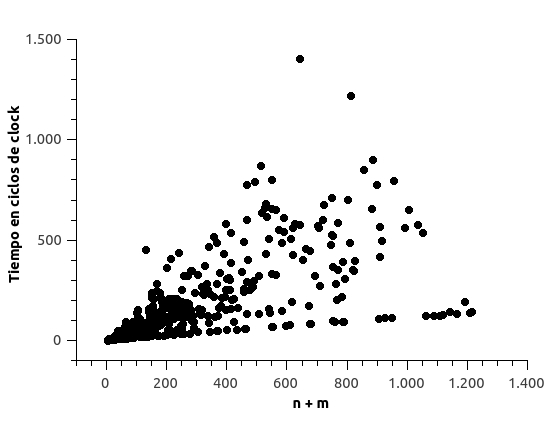
\includegraphics[width=\textwidth]{imagenes/ejer4-grafG2-1.jpg}
                \caption{Tiempos sin procesar}
        \end{subfigure}%
        ~ %add desired spacing between images, e. g. ~, \quad, \qquad, \hfill etc.
          %(or a blank line to force the subfigure onto a new line)
        \begin{subfigure}[b]{0.5\textwidth}
                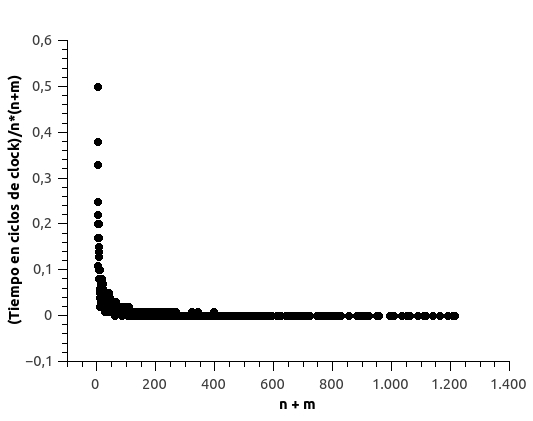
\includegraphics[width=\textwidth]{imagenes/ejer4-grafG2-2.jpg}
                \caption{figura (a) / n*(n+m)}
        \end{subfigure}
        
\end{figure}


\end{enumerate}

Como podemos ver de los 4 gráficos, al dividir los tiempos por $n*(n+m)$, tienden a un número constante mayor a cero. Entonces nuestro algoritmo tendría complejidad $\mathcal{O}(c*n*(n+m))$, donde $c$ es la constante a la cual converge el gráfico. Por lo tanto concluimos que la complejidad temporal experimental coincide con nuestra predicción de complejidad.


Por el lado de la calidad de las soluciones obtenidas con cada combinacion, debemos comparar por un lado el uso del BFS modificado o de la heuristica golosa como solucion inicial y por el otro el uso del primer criterio de vecindad o el del segundo criterio de vecindad como metodo de mejora de la solucion inicial:
\begin{itemize}
\item \textbf{BFS modificado vs Heuristica golosa como solucion inicial}. Para realizar la comparacion, tomamos el tamano de la solucion final para cada instancia, usando primero el BFS modificado como solucion incial y luego la heuristica golosa, para despues restar al tamano de la solucion final del tipo B1/B2, el tamano de la solucion final del tipo G1/G2. :

\begin{figure}[H]
        \centering
        \begin{subfigure}[b]{0.5\textwidth}
                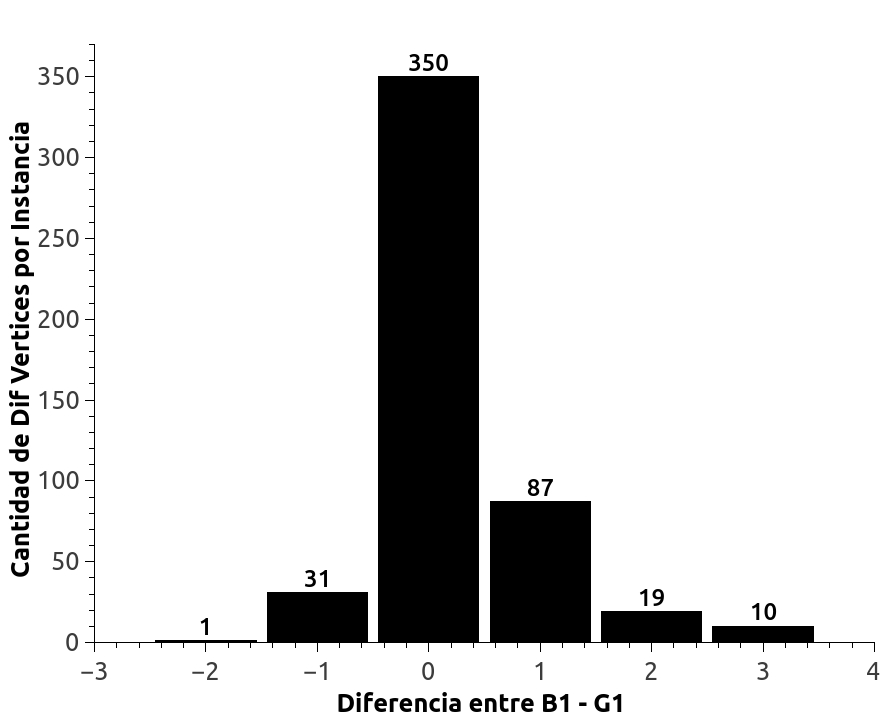
\includegraphics[width=\textwidth]{imagenes/ejer4-B1vsG1.jpg}
                \caption{Usando el Primer Criterio de Vecindad}
        \end{subfigure}%
        ~ %add desired spacing between images, e. g. ~, \quad, \qquad, \hfill etc.
          %(or a blank line to force the subfigure onto a new line)
        \begin{subfigure}[b]{0.5\textwidth}
                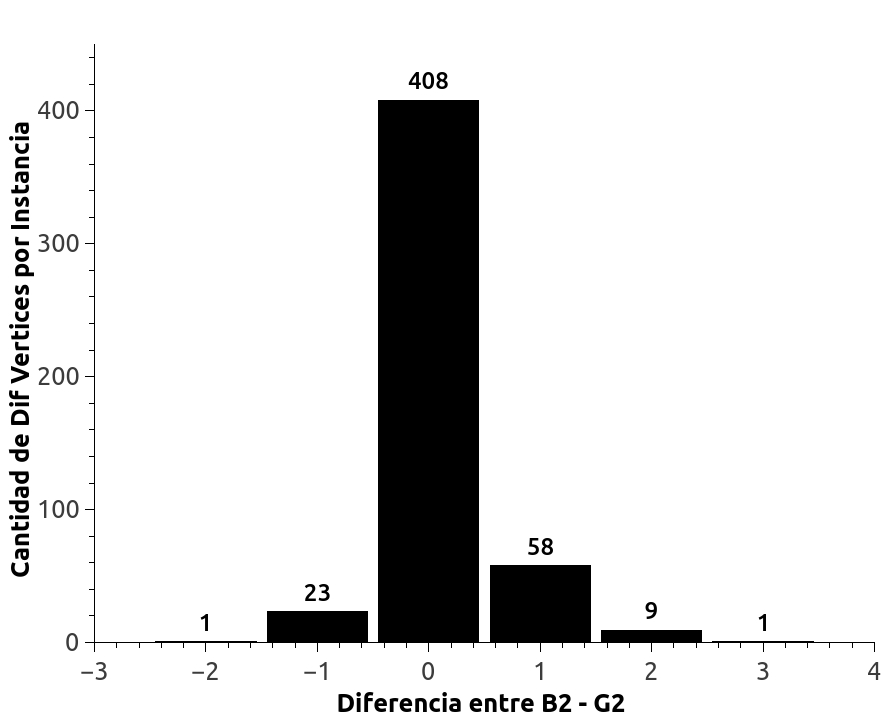
\includegraphics[width=\textwidth]{imagenes/ejer4-B2vsG2.jpg}
                \caption{Usando el Segundo Criterio de Vecindad}
        \end{subfigure}
        
\end{figure}

\end{itemize}

En ambos casos, se aprecia una paridad entre ambos soluciones, sin embargo hay una leve tendencia hacia la heuristica golosa como mejor procedimiento para construir la solucion inicial.

\begin{itemize}
	\item \textbf{Criterio de Vencindad}. El analisis comparado es el siguiente (utilizando la misma metodologia que en el caso de BFS vs Golosa):
    
    \begin{figure}[H]
        \centering
        \begin{subfigure}[b]{0.5\textwidth}
                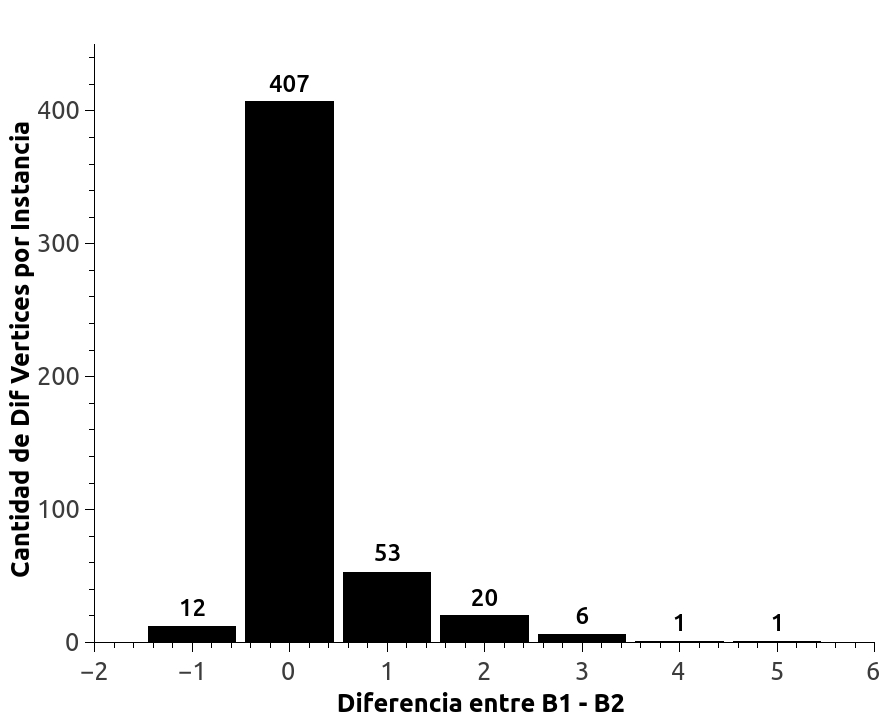
\includegraphics[width=\textwidth]{imagenes/ejer4-B1vsB2.jpg}
                \caption{Usando BFS como solucion incial}
        \end{subfigure}%
        ~ %add desired spacing between images, e. g. ~, \quad, \qquad, \hfill etc.
          %(or a blank line to force the subfigure onto a new line)
        \begin{subfigure}[b]{0.5\textwidth}
                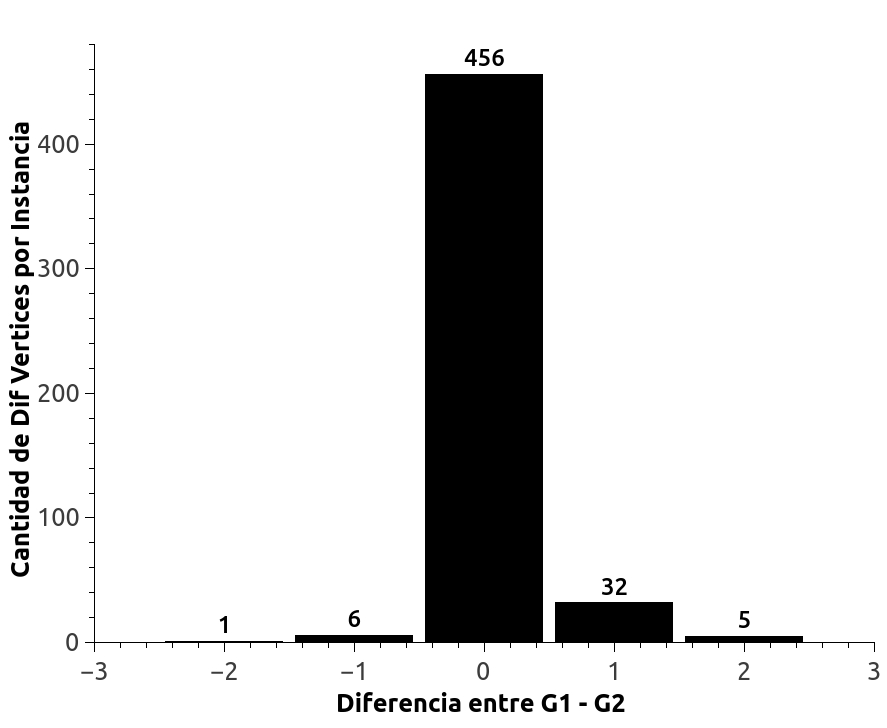
\includegraphics[width=\textwidth]{imagenes/ejer4-G1vsG2.jpg}
                \caption{Usando Goloso como solucion incial}
        \end{subfigure}
        
\end{figure}
    

\end{itemize}



Estos resultados nos inclinan a pensar que el segundo criterio de vecindad es el mejor criterio, lo cual es coherente con el hecho que el segundo criterio de vecindad es capaz de "arreglar" soluciones que el primer criterio de vecindad da como invalidas. Es decir, podriamos argumentar que como el primer criterio de vecindad es un caso particular del segundo criterio de vecindad (cuando no incluimos ningun vertice al subconjunto, mas alla del candidato) deberia ser siempre mejor al primero. Sin embargo, la experimentacion muestra casos donde el primer criterio es mejor, y eso se da en instancias donde arreglar una solucion invalida nos inhibe de seguir explorando la solucion original en busqueda de un mejor caso. Por ejemplo:

\begin{itemize}

	\item Grafo de n = 9 y m = 13
    
\tikz[every node/.style={draw,circle}] {
\node (1) at (0, 0)  { 1 };
\node (2) at (4.5, 0)  { 2 };
\node (3) at (2, -2)  { 3 };
\node (4) at (2, 2)  { 4 };
\node (5) at (7.5, -1.5)  { 5 };
\node (6) at (1, -1)  { 6 };
\node (7) at (3, 0)  { 7 };
\node (8) at (2.5, -1)  { 8 };
\node (9) at (4, -1)  { 9 };



\draw (1) edge node[above,draw=none] {} (6);
\draw (3) edge node[above,draw=none] {} (5);
\draw (4) edge node[above,draw=none] {} (6);
\draw (6) edge node[above,draw=none] {} (7);
\draw (6) edge node[above,draw=none] {} (3);
\draw (5) edge node[above,draw=none] {} (4);
\draw (7) edge node[above,draw=none] {} (4);
\draw (7) edge node[above,draw=none] {} (8);
\draw (9) edge node[above,draw=none] {} (8);
\draw (9) edge node[above,draw=none] {} (5);
\draw (9) edge node[above,draw=none] {} (2);
\draw (7) edge node[above,draw=none] {} (2);
\draw (8) edge node[above,draw=none] {} (3);


}

    
    
    \item \textbf{Solucion Golosa}: como el mayor grado, 3, es compartido por varios vertices, empezamos por el menor numero de etiqueta, que es el 5, y asi sucesivamente. 

\tikz[every node/.style={draw,circle}] {
\node (1) at (0, 0)  { 1 };
\node (2)[fill=blue!40, text=white] at (4.5, 0)  { 2 };
\node (3) at (2, -2)  { 3 };
\node (4) at (2, 2)  { 4 };
\node (5)[fill=blue!40, text=white] at (7.5, -1.5)  { 5 };
\node (6)[fill=blue!40, text=white] at (1, -1)  { 6 };
\node (7) at (3, 0)  { 7 };
\node (8)[fill=blue!40, text=white] at (2.5, -1)  { 8 };
\node (9) at (4, -1)  { 9 };



\draw (1) edge node[above,draw=none] {} (6);
\draw (3) edge node[above,draw=none] {} (5);
\draw (4) edge node[above,draw=none] {} (6);
\draw (6) edge node[above,draw=none] {} (7);
\draw (6) edge node[above,draw=none] {} (3);
\draw (5) edge node[above,draw=none] {} (4);
\draw (7) edge node[above,draw=none] {} (4);
\draw (7) edge node[above,draw=none] {} (8);
\draw (9) edge node[above,draw=none] {} (8);
\draw (9) edge node[above,draw=none] {} (5);
\draw (9) edge node[above,draw=none] {} (2);
\draw (7) edge node[above,draw=none] {} (2);
\draw (8) edge node[above,draw=none] {} (3);


}

    
    \item \textbf{Solucion aplicando el segundo criterio de vecindad a la solucion golosa}: tenemos 4 candidatos que cumplen con el hecho de tener 2 o mas adyacentes incluidos: 3, 4, 7, 9.
    \begin{enumerate}
    	\item Vertice 3: incluimos el 3, quitamos el 5, 6 y 8, por lo tanto podemos incluir un vertice mas, que sera el 1. Sin embargo el 4 no es dominado por nadie, por lo cual no es una solucion valida.
        \item Vertice 4: incluimos el 4, y quitamos el 5 y el 6. No podemos incluir ningun vertice mas, por lo tanto el 1 no es dominado por nadie, no es una solucion valida.
        \item Vertice 7: incluimos el 7 y quitamos el 2, 6 y 8. Incluimos el 1, y nos queda una solucion valida.
        \item Vertice 9: no es contemplado, ya que obtuvimos una solucion mejor con el vertice 7. Solucion que ya no es posible mejorar.
	\end{enumerate}
\tikz[every node/.style={draw,circle}] {
\node (1)[fill=blue!40, text=white] at (0, 0)  { 1 };
\node (2) at (4.5, 0)  { 2 };
\node (3) at (2, -2)  { 3 };
\node (4) at (2, 2)  { 4 };
\node (5)[fill=blue!40, text=white] at (7.5, -1.5)  { 5 };
\node (6) at (1, -1)  { 6 };
\node (7)[fill=blue!40, text=white] at (3, 0)  { 7 };
\node (8) at (2.5, -1)  { 8 };
\node (9) at (4, -1)  { 9 };



\draw (1) edge node[above,draw=none] {} (6);
\draw (3) edge node[above,draw=none] {} (5);
\draw (4) edge node[above,draw=none] {} (6);
\draw (6) edge node[above,draw=none] {} (7);
\draw (6) edge node[above,draw=none] {} (3);
\draw (5) edge node[above,draw=none] {} (4);
\draw (7) edge node[above,draw=none] {} (4);
\draw (7) edge node[above,draw=none] {} (8);
\draw (9) edge node[above,draw=none] {} (8);
\draw (9) edge node[above,draw=none] {} (5);
\draw (9) edge node[above,draw=none] {} (2);
\draw (7) edge node[above,draw=none] {} (2);
\draw (8) edge node[above,draw=none] {} (3);


}
    
    
    \item \textbf{Solucion aplicando el primer criterio de vecindad a la solucion golosa}: los candidatos son los mismos que en el segundo criterio, sin embargo al no poder incluir vertice mas alla del candidato, la solucion probando con el vertice 7 es invalida, ya que el 1 no es dominado por nadie. Por lo tanto probamos con incluir el 9, y quitar el 2, 5 y 8. Al hacer esto nos queda una solucion valida de menor cardinal que en la solucion golosa original y que si hubiesemos utilizado el segundo criterio



\tikz[every node/.style={draw,circle}] {
\node (1) at (0, 0)  { 1 };
\node (2) at (4.5, 0)  { 2 };
\node (3) at (2, -2)  { 3 };
\node (4) at (2, 2)  { 4 };
\node (5) at (7.5, -1.5)  { 5 };
\node (6)[fill=blue!40, text=white] at (1, -1)  { 6 };
\node (7) at (3, 0)  { 7 };
\node (8) at (2.5, -1)  { 8 };
\node (9)[fill=blue!40, text=white] at (4, -1)  { 9 };



\draw (1) edge node[above,draw=none] {} (6);
\draw (3) edge node[above,draw=none] {} (5);
\draw (4) edge node[above,draw=none] {} (6);
\draw (6) edge node[above,draw=none] {} (7);
\draw (6) edge node[above,draw=none] {} (3);
\draw (5) edge node[above,draw=none] {} (4);
\draw (7) edge node[above,draw=none] {} (4);
\draw (7) edge node[above,draw=none] {} (8);
\draw (9) edge node[above,draw=none] {} (8);
\draw (9) edge node[above,draw=none] {} (5);
\draw (9) edge node[above,draw=none] {} (2);
\draw (7) edge node[above,draw=none] {} (2);
\draw (8) edge node[above,draw=none] {} (3);


}

\end{itemize}

Sin embargo estos tipos de instancias son muy particulares, por lo cual podemos afirmar que la \textbf{mejor combinacion} para la \textbf{heuristica de busqueda local} planteada es aquella que toma como \textbf{solucion inicial} la generada por la \textbf{heuristica golosa} y luego es mejorada por el \textbf{segundo criterio de vecindad}.











